\chapter{Stavba siete} \label{stavba}

Všetky siete boli napísané v programovacom jazyku \textit{Python} s použitím knižníc \textit{numpy} a \textit{tensorflow}.
V prípade futbalu bola na začiatku sieť skonštruovaná so všetkými 44 príznakmi, ktoré sme dostali z transformačnej časti práce (Príloha \ref{in:foot}).
Sieť teda obsahovala vstup o veľkosti 44 príznakov, 2 skryté vrstvy neurónov (s 25, resp. 15 neurónmi) a troj-neurónový výstup typu softmax, ktorý vyberie najpravdepodobnejšiu možnosť, nastaví daný výstup neurónu na 1 a zvyšné nastaví na 0.
V prípade tenisu bola sieť skonštruovaná so všetkými 37 príznakmi (ich popis je Príloha \ref{in:ten}) a taktiež obsahovala 2 skryté vrstvy neurónov s rovnakým počtom neurónov na nich ako v prípade futbalu. Výstup predstavoval dva neuróny, na ktoré bol opäť použitý softmax, ktorý vyberie najvyššiu hodnotu.
Na vylepšovanie siete sme, ako je napísané v jednej z predošlých kapitol (\ref{docu}), použili údaje, ktoré sa napokon budú pri vyhodnocovaní nachádzať medzi testovacími datami. 

Konkrétne, pre futbal data predstavovali 7 celých sezón a prvú polovicu ďalšej sezóny (ako popísané v \ref{foot}), vyhodnocovacie data predstavujú teda druhú polovicu tejto sezóny. 
Takže sme trénovacie data rozdelili na tri časti, 6 celých sezón a polovicu ďalšej (trénovacie data), druhú polovicu siedmej sezóny (testovacie data) a zvyšnú prvú polovicu ôsmej sezóny (nepoužité data).
V prípade tenisu prišli data už priamo z transformačnej časti v troch súboroch, trénovacie, testovacie a vyhodnocovacie data.

Každá sieť mala svoje nedostatky v celkovej úspešnosti, ale doposiaľ neexistuje efektívne nastavenie neurónových sietí pre každú situáciu \citep{gitgud}, takže každá sieť sa musela vylepšovať osobitne a manuálne vzhľadom na rozdiely v prístupoch.
Cieľom práce nie je porovnať rovnakú architektúru a viac typov neurónových sietí, ale pokúsiť sa získať, čo možno najlepšie výsledky a porovnať potenciály doprednej a rekurentnej neurónovej siete.

\section{Selekcia príznakov}
Kliatba dimenzionality nám hovorí, že čím viac vstupných príznakov zadáme neurónovej sieti, tým sú data redšie a teda je ich potreba získať viac, aby sa sieť správne učila. Viac dat získať nevieme, takže sa pokúsime znížiť počet dimenzií a pozrieť sa na to, ako sa to prejaví na trénovacích datach.
Na začiatok spravíme korelačný test všetkých príznakov testovacích a trénovacích dat (obrázky \ref{corr} a \ref{corr_atp}).
Teória hovorí, že by nám mohla napovedať, aké hodnoty sú dôležité.
Obrázok hovorí, že najvyššiu koreláciu s výsledkom zápasu majú príznaky 41 a 42 určujúce dlhodobú silu tímu. Skóre dosahuje tiež celkom vysokú koreláciu (okolo 0,2) s finálnym výsledkom.
V prípade tenisu obrázok naznačuje najvyššiu koreláciu medzi výsledkom a oboma druhmi skóre, veľkú rolu zohráva postavenie v rebríčku ATP a vzájomné zápasy (konkrétne priemerný rozdiel v počte vyhraných gemov za set).

\noindent
\begin{figure} \label{corr}
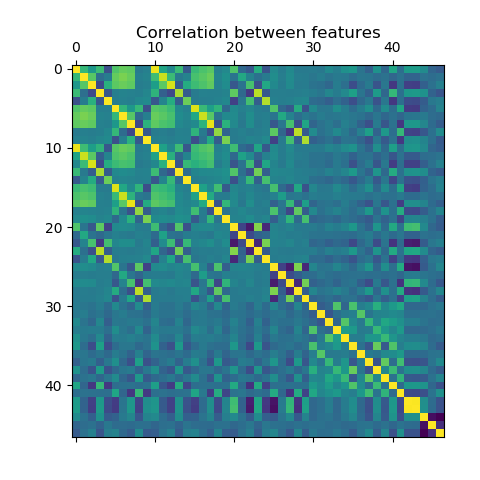
\includegraphics[scale=0.9]{../img/correng.png}
\caption{Korelačná tabuľka všetkých príznakov pre anglickú Premier League, žltá predstavuje kladnú koreláciu, modrá zápornú. Nás hlavne zaujímajú posledné 3 riadky určujúce koreláciu príznaku s výsledkom zápasu (príznaky sú v poradí ako v Prílohe \ref{in:foot}).}
\end{figure}
\begin{figure} \label{corr_atp}
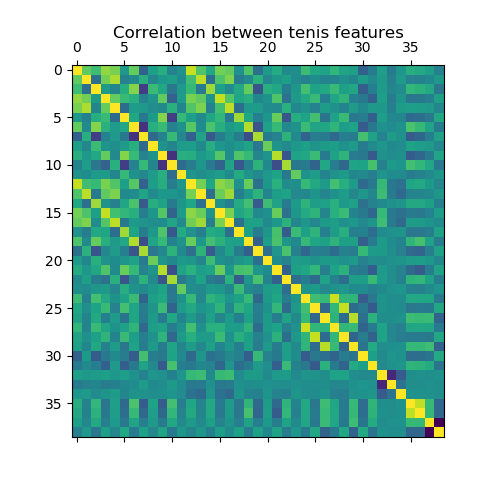
\includegraphics[scale=0.9]{../img/corratp.png}
\caption{Korelačná tabuľka všetkých príznakov pre tenisové zápasy, žltá predstavuje kladnú koreláciu, modrá zápornú. Nás hlavne zaujímajú posledné 2 riadky určujúce koreláciu príznaku s výsledkom zápasu (príznaky sú v poradí ako v Prílohe \ref{in:foot}).}
\end{figure}

Tieto tabuľky boli pre nás viac-menej informačné. 
Selekcia príznakov, s ktorými dosahovala sieť najlepšie trénovacie výsledky a ktoré budú použité na získanie výsledkov v kapitole \ref{res}, bol uskutočnený spôsobom pokus-omyl, keďže nič lepšie nevieme, ako už bolo spomínané na začiatku kapitoly.

\section{Výsledky tréningu}
Pri trénovaní siete boli pre každú množinu príznakov prenastavované aj iné parametre siete, pri snahe získať čo najlepšie výsledky.
Iba pre tréning doprednej neurónovej siete na predikciu futbalu predstavoval viac ako 100 rôznych vyskúšaných modelov siete, celkový počet vyskúšaných modelov bol okolo 250.
Tabuľky \ref{ff_train_res} a \ref{rnn_train_res} predstavujú nastavenia jednotlivých parametrov siete, pri ktorých dosahovali dopredné, resp. rekurentné neurónové siete najlepšie výsledky.

\begin{table}[h]
\begin{center}
\begin{tabular}{ p{7em}|c|c|c|c|c|c|c|c|c|c| } 
 Predpovedaný šport (liga) & \multicolumn{6}{|c|}{Parametre siete} & \multicolumn{4}{|c|}{Trénovacie výsledky}  \\ 
 \hline
  & O & B & LR & E & $H_1$ & $H_2$ & TrA\% & TeA\% & CG\% & CGP \\
 \hline \hline
 0 & 0 & 0 & 0 & 0 & 0 & 0 & 0 & 0 & 0 & 0 \\ 
 0 & 1 & 1 & 0 & 0 & 0 & 0 & 0 & 0 & 0 & 0 \\ 
 1 & 0 & 1 & 0 & 0 & 0 & 0 & 0 & 0 & 0 & 0 \\ 
 1 & 1 & 0 & 0 & 0 & 0 & 0 & 0 & 0 & 0 & 0 \\ 
 \hline
\end{tabular}
\caption{Tabuľka funkcie XOR}
\label{ff_train_res}
\end{center}
\end{table}

\begin{table}[h]
\begin{center}
\begin{tabular}{ p{7em}|c|c|c|c|c|c|c|c|c|c|c|c| } 
 Predpovedaný šport (liga) & \multicolumn{8}{|c|}{Parametre siete} & \multicolumn{4}{|c|}{Trénovacie výsledky}  \\ 
 \hline
  & O & B & LR & E & $H_1$ & $H_2$ & N & T & TrA\% & TeA\% & CG\% & CGP \\
 \hline \hline
 0 & 0 & 0 & 0 & 0 & 0 & 0 & 0 & 0 & 0 & 0 & 0 & 0 \\ 
 0 & 1 & 1 & 0 & 0 & 0 & 0 & 0 & 0 & 0 & 0 & 0 & 0 \\ 
 1 & 0 & 1 & 0 & 0 & 0 & 0 & 0 & 0 & 0 & 0 & 0 & 0 \\ 
 1 & 1 & 0 & 0 & 0 & 0 & 0 & 0 & 0 & 0 & 0 & 0 & 0 \\ 
 \hline
\end{tabular}
\caption{Tabuľka funkcie XOR}
\label{rnn_train_res}
\end{center}
\end{table}